\documentclass[border=4pt]{standalone}
% Preámbulo común de las figuras. Cada figura es un documento standalone
% que se compila a SVG con scripts/build_figures.sh
\usepackage[utf8]{inputenc}
\usepackage{amsmath}
\usepackage{tikz}
\usepackage[american, siunitx]{circuitikz}
\usetikzlibrary{arrows.meta,calc,decorations.pathmorphing,patterns}
\tikzset{
  >={Stealth[length=2.2mm]},
  eje/.style={->, thin},
  hilo/.style={thick},
}
% Paleta común: tonos medios legibles sobre fondo claro
\definecolor{azul}{RGB}{31,94,168}
\definecolor{rojo}{RGB}{192,57,43}
\definecolor{verde}{RGB}{39,128,73}
\definecolor{naranja}{RGB}{211,120,30}
\definecolor{morado}{RGB}{125,60,152}

\begin{document}
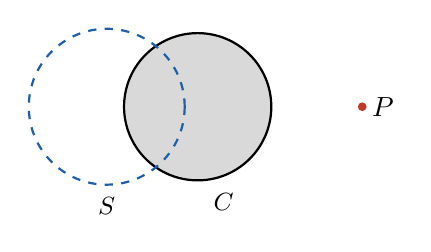
\begin{tikzpicture}[scale=1.1]
  \filldraw[fill=gray!30, draw=black, thick] (0.45,0) circle (0.85);
  \draw[thick, dashed, azul] (-0.6,0) circle (0.9);
  \fill[rojo] (2.35,0) circle (0.05) node[right, text=black]{$P$};
  \node[font=\small] at (-0.6,-1.15) {$S$};
  \node[font=\small] at (0.75,-1.1) {$C$};
\end{tikzpicture}
\end{document}
